\newpage
\sect{3 \quad Identified limitation and hypothesis}
\textbf{Challenge.} To cluster by digit identity, the embedding should distinguish a 7 from a 2. A decoder can also reduce its pixel error by drawing a triangle in the margin [1,4]. Uniform reconstruction gives one unit of squared error on that triangle the same cost as one unit on a digit stroke. We hypothesize that this incentive can impair digit clustering. Random geometry alone could also make clustering harder.

\begin{center}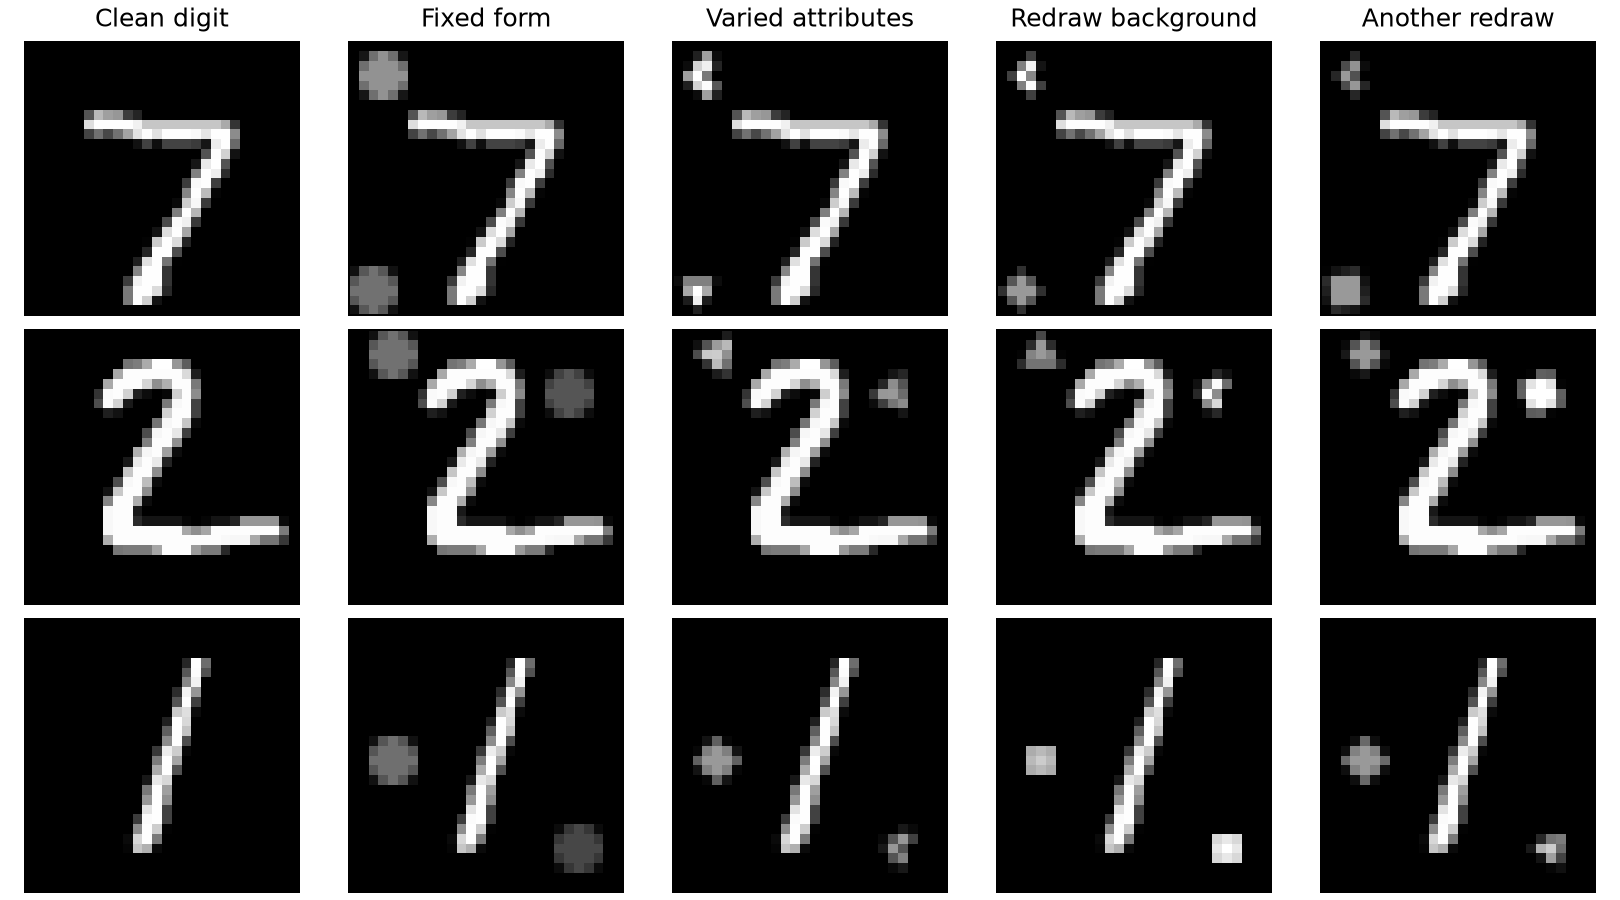
\includegraphics[width=.67\linewidth]{../figures/varied.png}\end{center}
\smallcap{\textbf{Figure 1.} The same MNIST handwriting across each row. The generator places two symbols in disjoint $5\times5$ boxes and preserves each nonzero stroke pixel plus a one-pixel clearance. The last three columns redraw symbol attributes at the same two positions.}

\textbf{Philosophy.} Give the decoder a stronger reason to preserve features that determine the intended grouping. MNIST digits are centered, so we use location as an imperfect estimate of relevance. It is available from a single observed image, including at training time.

\sect{4 \quad Proposed modification to the reconstruction loss}
For pixel $j$ at position $p_j$, let $v_j=\exp(-\|p_j-(13.5,13.5)\|^2/(2\cdot7^2))$ and $w_j=v_j/\bar v$. Replace uniform MSE with
\[
L_G(x,\hat x)=\frac{1}{784}\sum_{j=1}^{784}w_j(\hat x_j-x_j)^2 .
\]
The map has mean one. A central and a peripheral error of the same magnitude now have different costs. Our proposed IDEC applies $L_G$ in both autoencoder pretraining and clustering. A stage ablation applies it in each stage alone. Training uses the observed image as the target and the same fixed weights for every image.

\begin{center}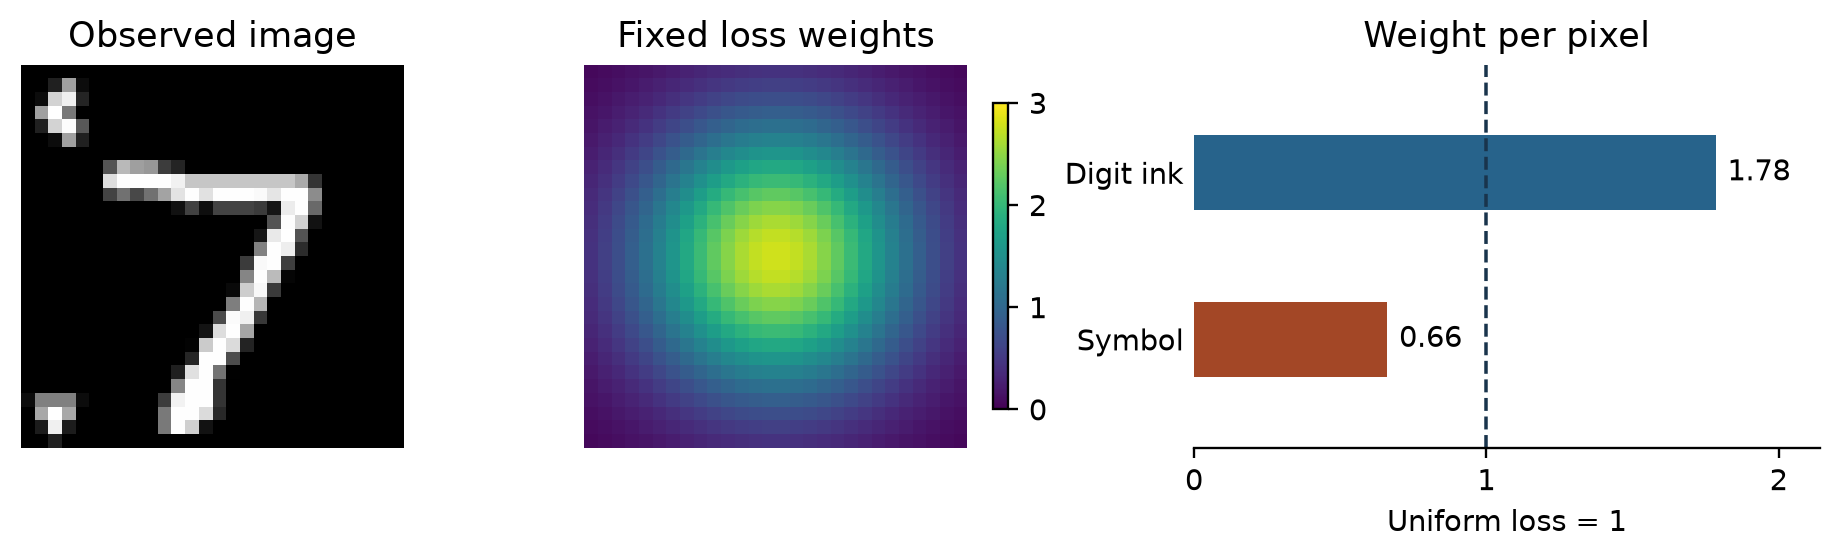
\includegraphics[width=.87\linewidth]{../figures/gaussian_prior.png}\end{center}
\smallcap{\textbf{Figure 2.} The model sees the marked image. We used the generator only to audit where the weights fall. Across training pixels the mean was 1.78 on ink and 0.66 on symbols. A central symbol still receives a large weight.}

\newpage
\sect{5 \quad Experimental setup}
Use the same 12,000 training digits and 10,000 held-out digits in both domains [5]. The marked domain contains two symbols from 96 combinations of shape, radius, angle and grayscale brightness. Attributes are assigned by a balanced shuffle independent of digit labels. Each training digit keeps its background. Held-out digits receive independently generated symbols under the same rules.

\textbf{Matched models.} Within each domain and seed (0--4), train a $784$--$500$--$500$--$2000$--$10$ autoencoder for 100 epochs and run K-means with 20 restarts. Fork the very same weights and centers. DEC minimizes only $0.1\,\mathrm{KL}(P\Vert Q)$ during clustering [2]. Ordinary IDEC adds uniform MSE. A third fork adds $L_G$. Gaussian pretraining provides another shared starting point for uniform or Gaussian fine-tuning. The fixed KL multiplier, Adam learning rate $10^{-3}$, batch size 256, target refresh every 140 updates and 5,600 updates match across all forks. Our controlled implementation uses a plain autoencoder for initialization. A separate KL-only control skips pretraining entirely and starts from a random encoder. This control spends fewer training updates.

\textbf{Primary comparison.} For method $m$ and seed $s$, compute $D_{m,s}=\mathrm{ACC}_{m,s}^{\rm clean}-\mathrm{ACC}_{m,s}^{\rm marked}$ in percentage points. Both scores use matching training and test domains and the same digit identities. A positive $D_{\rm IDEC,s}-D_{\rm DEC,s}$ means IDEC lost more. $D_{\rm IDEC,s}-D_{\rm Gaussian,s}$ measures whether weighting reduced IDEC's background penalty after accounting for its effect on clean digits. Fit the cluster-to-digit map on training predictions after fitting and freeze it for every test view. The quantity after $\pm$ is the sample SD across five paired seeds. The \href{https://github.com/JohnR31N/cs126FinalProj/blob/7e753dd/IDEC/dec_background/design.md}{follow-up protocol} predates the DEC fits.

\sect{6 \quad Testing the incentive to reproduce background symbols}
An earlier experiment held the marked inputs fixed and supplied either the marked image or the original clean digit as the reconstruction target [6]. With the clean target, copying a symbol incurs an error because its target pixels are zero. This changes the reconstruction task using privileged information from the generator. Separately, circles matched to the varied symbols in number, position and squared intensity gave 65.74\% ACC, close to the 65.40\% with varied geometry. Extra harm from geometric diversity itself was inconsistent across seeds.

\begin{center}\small\begin{tabular}{llrrr}
\toprule
Pretrain target & Fine-tune target & Marked ACC & Redraw flips & Decoder response\\
\midrule
Full & Full & 65.40 & 2.98 & 0.00828\\
Full & Clean & 66.85 & 2.65 & 0.00159\\
Clean & Full & 70.62 & 2.51 & 0.00289\\
Clean & Clean & 71.44 & 2.35 & 0.00145\\
\bottomrule
\end{tabular}
\end{center}
\smallcap{\textbf{Table 2.} Earlier target ablation on identical marked inputs. ACC and flips are percentages. Flips count cluster changes when only the symbol attributes are redrawn. Decoder response projects the change in reconstruction onto the change in input, with one denoting full tracking.}
Using clean targets in both stages gained $6.04\pm4.37$ points of marked ACC. All five seeds gained accuracy and showed lower decoder response. Changing only the pretraining target gained 5.23 points on average, compared with 1.45 for changing only the fine-tuning target. This supports an effect of what the decoder must reproduce and motivates measuring the initialization as well as the final clusters.

\newpage
\sect{7 \quad Results of the matched DEC and IDEC comparison}
\begin{center}\small\setlength{\tabcolsep}{5pt}\begin{tabular}{lrrrr}
\toprule
Method & Clean ACC & Marked ACC & Drop (pp) & Redraw flips\\
\midrule
DEC & 77.63 & 70.86 & 6.77 $\pm$ 5.40 & 3.19\\
IDEC & 73.23 & 65.14 & 8.09 $\pm$ 5.01 & 2.99\\
DEC + translation & 81.36 & 77.18 & 4.17 $\pm$ 4.04 & 2.34\\
IDEC + translation & 83.88 & 77.61 & 6.27 $\pm$ 2.74 & 1.78\\
Gaussian, both stages & 70.03 & 65.59 & 4.44 $\pm$ 3.98 & 2.63\\
Gaussian, pretraining only & 74.07 & 68.80 & 5.27 $\pm$ 4.64 & 2.62\\
Gaussian, fine-tuning only & 69.27 & 62.88 & 6.39 $\pm$ 5.18 & 3.20\\
KL only, random start & 31.00 & 28.90 & 2.10 $\pm$ 1.75 & 11.42\\
\bottomrule
\end{tabular}
\end{center}
\smallcap{\textbf{Table 3.} Clean and marked ACC use matching training and test domains. The drop is clean minus marked ACC, computed before rounding (mean $\pm$ paired seed SD in points). Flips use marked-trained models. The two translation rows add 20 fits to the 60 fixed control fits. The translated DEC and IDEC branches share a pretrained encoder and centers within each seed and domain.}
\textbf{Does continuing reconstruction cost more?} Both models lost accuracy in all five seeds. DEC fell from 77.63\% to 70.86\%, and IDEC fell from 73.23\% to 65.14\%. The IDEC-minus-DEC differences in loss were $+2.78,-3.88,+1.77,+5.22,+0.71$ points. The mean was $+1.32\pm3.35$ points. DEC also reached higher absolute ACC in both domains in every seed. All ten clusters were occupied for both methods.

\textbf{Where sensitivity appears.} Before either fork started clustering, the shared uniform autoencoder plus K-means already scored 73.42\% clean and 68.22\% marked, a 5.20-point drop. In a separate test-time intervention, adding symbols to the test images of a frozen clean-trained model cost 2.01 points for DEC and 8.62 for IDEC. That comparison fixes the model, whereas Table~3 changes the training and test domains together.

\textbf{What the Gaussian changed.} Weighting both stages reduced the background drop by $3.65\pm5.43$ points in the paired comparison (four of five seeds). Marked accuracy gained only $0.45\pm4.76$ points, improving in three seeds. Clean accuracy fell by $3.20\pm2.38$ points, declining in all five. Thus most of the smaller gap came from a weaker clean baseline. On marked-trained models, redraw flips fell from 2.99\% to 2.63\%, and decoder response fell from 0.00843 to 0.00529. Both decreased in every seed.

\textbf{What whole-image translation changed.} Translated IDEC gained 12.47 points on marked digits and 10.65 on clean digits, relative to ordinary IDEC. Both improved in every seed. The background drop shrank by $1.82\pm3.70$ points in the paired comparison, with three reductions and two increases. Redraw flips fell from 2.99\% to 1.78\% in the mean, lower in every seed. Translated DEC gained 6.33 points on marked digits and 3.73 on clean digits. With translation in both methods, IDEC still lost $2.10\pm1.47$ points more accuracy to the symbols than DEC did, in the same direction in all five seeds.


\begin{center}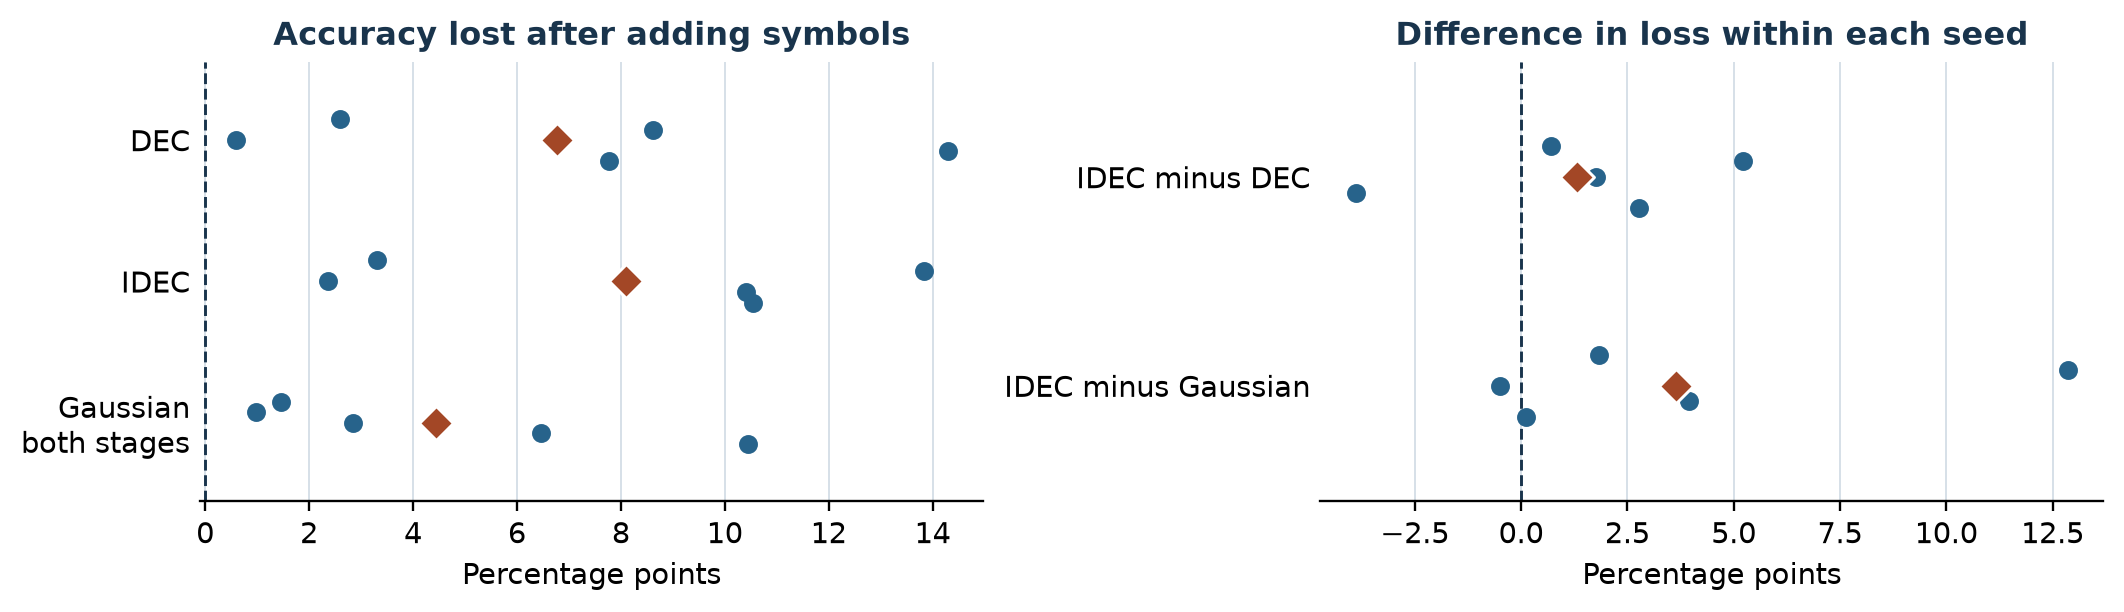
\includegraphics[width=.98\linewidth]{../figures/dec_background_drops.png}\end{center}
\smallcap{\textbf{Figure 3.} Blue dots represent the five seeds and orange diamonds their means. On the right, a positive difference means ordinary IDEC lost more accuracy than the named comparison method. Subtracting within each seed preserves the pairing.}

\newpage
\sect{8 \quad Limitations and conclusion}
\textbf{What supports the proposed limitation.} Holding marked inputs fixed and changing their reconstruction targets improved digit clustering in every seed. Adding the geometry hurt DEC as well as IDEC. Some of the performance loss was already present at their shared initialization. Keeping the reconstruction term during clustering was associated with a modest additional mean loss in this comparison, with a reversal in one seed. The experiment supports a contribution from the reconstruction objective while leaving the fraction of the accuracy loss attributable to background encoding unresolved.

\textbf{Where to apply the spatial prior.} Among the three Gaussian placements, weighting only pretraining gave the highest marked accuracy (68.80\%). Its marked gain of $3.66\pm4.74$ points over IDEC was positive in four seeds, with a mean clean gain of 0.84 points. Weighting only fine-tuning reduced marked ACC by $2.26\pm1.29$ points even though its decoder response also fell, to 0.00480. For centered digits, the pretraining-only variant offers the best observed tradeoff among the weighted objectives. This is a stage-ablation finding on the same split. The prespecified two-stage variant had a small, inconsistent gain in marked accuracy.

\textbf{Skipping reconstruction entirely.} With a random encoder, KL-only clustering scored 31.00\% clean and 28.90\% marked. In seed 4 both domains collapsed to one cluster (11.35\% ACC). A 2.10-point mean drop from this low baseline gives little evidence of useful robustness. The standard DEC comparison in Table~3 uses a trained encoder and retains all ten clusters.


The prior assumes that central pixels generally matter more to digit identity. A symbol near the center gets a high reconstruction weight, and an off-center stroke gets a low one. On MNIST the available sites depend on the digit silhouette. The two small grayscale marks, a single image split and five model seeds limit transfer to other backgrounds and data distributions. A decoder response measures only the information used to render the changed pixels. It leaves open how much background information the encoder retains for other purposes.

\textbf{Augmentation control.} The \href{https://github.com/JohnR31N/cs126FinalProj/blob/c22ae3d/IDEC/dec_background/translation/design.md}{translation addendum} moves the entire image within three pixels on each axis during pretraining. The input and reconstruction target undergo the same shift. Omitting a symbol incurs the same uniform squared error at its new position. Fine-tuning uses the unshifted images. Keeping every stroke and symbol in frame permits an average of 45.5 legal offsets on clean training images and 23.9 on marked images, out of 49 possible. This changes the strength of augmentation across domains. Redraw flips measure the final decision's sensitivity to the background. A lower rate leaves open what the encoder remembers about the symbols.
